%----------------------------------------------------------------------------------------
%       CHAPTER 3
%----------------------------------------------------------------------------------------

\cleardoublepage

\chapterimage{amoc.png} % Chapter heading image

\chapter{Ocean circulation}\label{ch:ocean-circulation}

\hfill \break

\noindent Stuff to keep in mind:

\begin{itemize}
\item Nothing at all – keep your mind completely empty and let the wonderful truths of \textbf{muffin} permeate your entire being.
\end{itemize}

\vspace{2mm}
\noindent Background reading (Atlantic circulation and stability in \textbf{muffin}):

\vspace{2mm}
\begin{itemize}
\item Hargreaves et al. [2004] (Climate Dynamics 23, 2004, Pages 745 – 760)
\\\(\rightarrow\)Simple assessment of the likelihood of AMOC collapse.
\item Marsh et al. [2004] (Climate Dynamics, 23 2004, Pages 761 – 777)
\\\(\rightarrow\)Characterization of thresholds of AMOC collapse.
\item Singaraye et al. [2008] (GRL 35, doi:10.1029/2008GL034074)
\\\(\rightarrow\)Role of changing ocean circulation in atmospheric radiocarbon variability during the Younger Dryas.
\end{itemize}

\vspace{2mm}
\noindent Background reading (Miscellaneous (model) Atlantic circulation and stability):

\vspace{2mm}
\begin{itemize}
\item IPCC [2007] (e.g., Section 10.3.4)
\\\(\rightarrow\)Future predictions of AMOC strength.
\item Schmittner [2005] (Nature 434, 628– 633)
\\\(\rightarrow\)Impacts on marine ecosystems and carbon cycling.
\item Obata [2007] (J. Clim. 20, 5962–5976)
\\\(\rightarrow\)Climate-carbon cycle model response to freshwater discharge.
\end{itemize}

%------------------------------------------------
\newpage
%------------------------------------------------

\section*{READ.ME}

You will need to download a new \textit{re-start} file prior to embarking on the experiments with modern ocean circulation.
To fetch this: change to the \texttt{cgenie\_output} directory, and type (or copy and paste carefully from the PDF ...):

\vspace{-2mm}
\small\begin{verbatim}
$ wget --no-check-certificate http://www.seao2.info/cgenie_output/LAB_2.SPIN.tar.gz
\end{verbatim}\normalsize
\vspace{-2mm}

This downloads an archived/compressed copy of the 10,000 year \textit{spin-up} experiment \texttt{LAB\_2.SPIN}. Extract the contents of this archive by typing:

\vspace{-2mm}
\begin{verbatim}
$ tar xfzv LAB_2.SPIN.tar.gz
\end{verbatim}
\vspace{-2mm}

You’ll then need to change directory back to \texttt{genie-main} to run the model.

%------------------------------------------------
\newpage
%------------------------------------------------

\section{Visualizing ocean circulation}

Visualizing the 3D flow (/transport) of the ocean, much less the rate at which this occurs, is no trivial matter. Even with the aid of a model. (Or rather, the problem then becomes: how to visualize ocean circulation in a model.) We'll consider two different ways of analysing model velocity fields first -- simply utilizing the \textit{restart} that you have downloaded and unpacked, and then later take a more pro-active approach in subsequent Sections with some new experiments.

\vspace{1mm}
\noindent\rule{4cm}{0.5pt}
\vspace{2mm}

\noindent The first approach we can take is to simply visualize the raw velocity fields, but plotted as ocean currents.\vspace{1mm}
\begin{enumerate}[noitemsep]
\vspace{1mm}
\item  In the 3D \textbf{netCDF} file, the three components of ocean velocity are represented by the variables: ocean velocity – u (Eastwards), ocean velocity – v (Northwards), and ocean velocity – w (upwards). 2. Open up velocity – u. Chose ‘lon-lat’.
\vspace{1mm}
\item Select/highlight velocity – v. and click on the ‘Combine Plot’ icon (as per before).
\vspace{1mm}
\item Rather than a difference map, which is what you get by default, i.e., ‘Array 1 – Array 2’ – from the drop-down menu (next to the ‘Interpolate’ button) select ‘Vector Magnitude’.
\vspace{1mm}
\item You should have a color contoured (or not if you prefer plotting without contouring on) map of ocean current speed, with velocity vectors (direction and magnitude) overlain. You’ll need to re-scale the velocity vectors to properly see them – from the ‘Contours and Vectors’ tab – change the ‘Scale Length’ to e.g., 0.1. (On a \textbf{Mac}, look under the ‘Vectors’ tab for a ‘Reference Value’ to something like 0.1.)  When fresh-water hosing – look out for impacts on the N. Atlantic current system associated with the AMOC.
\vspace{1mm}
\item You can repeat this for deeper depth levels in the ocean – e.g., between about 1500 and 2000 m is a good place to go looking for the Western boundary current (and AMOC return) in the model (such as it exists at this low resolution) but you’ll need to re-scale the velocity vectors again (e.g., to 0.01 to less).
\end{enumerate}
\vspace{1mm}

\noindent An example plot (using \textbf{Panoply} for visualizing surface ocean current fields) is given in Figure \ref{fig:ch3-currents1}.

\begin{figure}
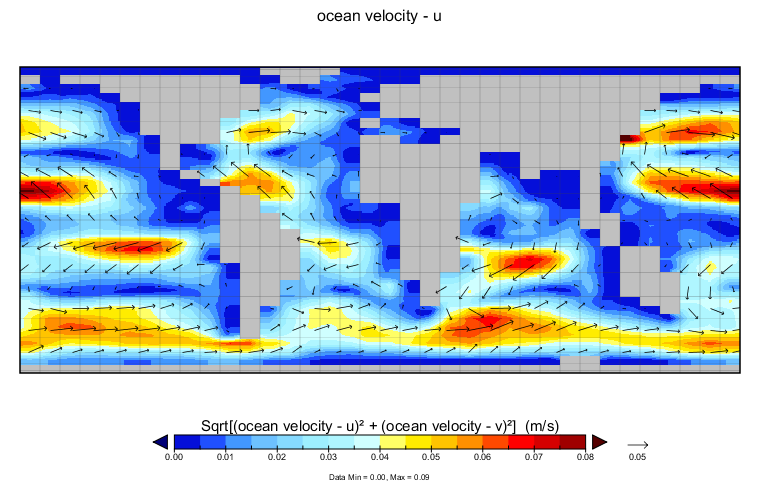
\includegraphics[width=0.6\textwidth]{ch3-currents1.png}\centering
\vspace{-0mm}
\caption{Example plot of (normal/default modern) ocean current fields (3D netCDF file). Again scaling has been set manually to create an easy-to-interpret axis scale. On the left is the surface field, and on the right an intermediate depth (illustrating what approximates the Deep Western Boundary current in the model in the Atlantic).}
\label{fig:ch3-currents1}
\end{figure}

%------------------------------------------------
\vspace{1mm}
\noindent\rule{4cm}{0.5pt}
\vspace{2mm}
%------------------------------------------------

\noindent The second approach is to visualize the large-scale ocean transport in terms of the meridional overturning circulation ('stream-function') (e.g. see background literature).

Two example plots (using \textbf{Panoply}) are shown in Figure \ref{fig:ch3-amoc1} for the Atlantic basin, and Figure \ref{fig:ch3-amoc2} for the Pacific. In the In the 2D \textbf{netCDF} file, relevant fields (netCDF variables)\footnote{Note that these fields are only meaningful for the modern arrangement of the continents and a continuous separation of the Atlantic from the Pacific from high northern latitudes down to the tip of South America. Different (e.g. paleo) arrangements of the continents may not have recognisable (or definable) Atlantic and/or Pacific basins and it may only be possible to define and visualize the global meridional overturning circulation -- variable: \textsf{\footnotesize phys\_opsi}.} are:
\begin{itemize}[noitemsep]
\setlength{\itemindent}{.0in}
\item [] \textsf{\footnotesize phys\_opsia} == global overturning stream-function
\item [] \textsf{\footnotesize phys\_opsip} == overturning in the Atlantic
\end{itemize}

\begin{figure}
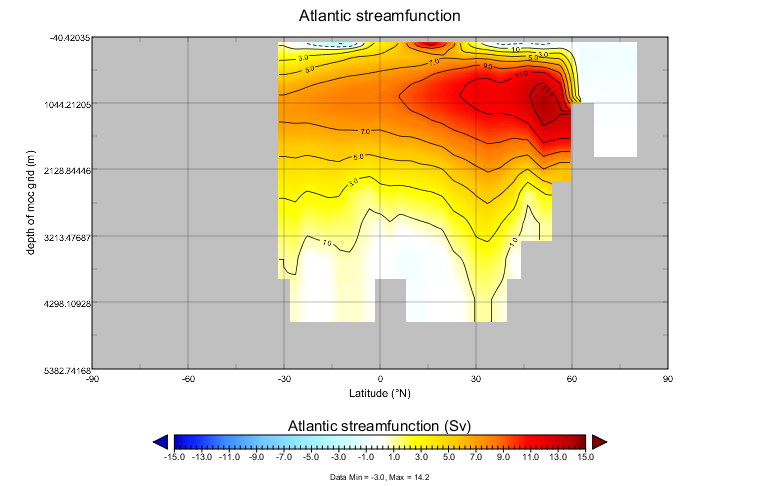
\includegraphics[width=0.6\textwidth]{ch3-amoc1.png}\centering
\vspace{-0mm}
\caption{Example plot of (normal/default modern) overturning stream-function (2D \textbf{netCDF} file). (e.g., for Atlantic: \textbf{netCDF} parameter name: \texttt{phys\_opsia}, long-name: Atlantic stream-function). Note that auto-scaling has been turned off and the min and max plotting limits set manually. By convention, stream-functions are plotted with their scale symmetrical around zero, giving red and ‘warm’ colors for positive value and clockwise overturning, and blues and ‘cold’ colors for negative values and anti-clockwise overturning. (The plot has been tart-ed up by overlaying solid contours plus contour labels.) It may be necessary in \textbf{Panoply} to re-orient (invert) the vertical grid.}
\label{fig:ch3-amoc1}
\end{figure}

\begin{figure}
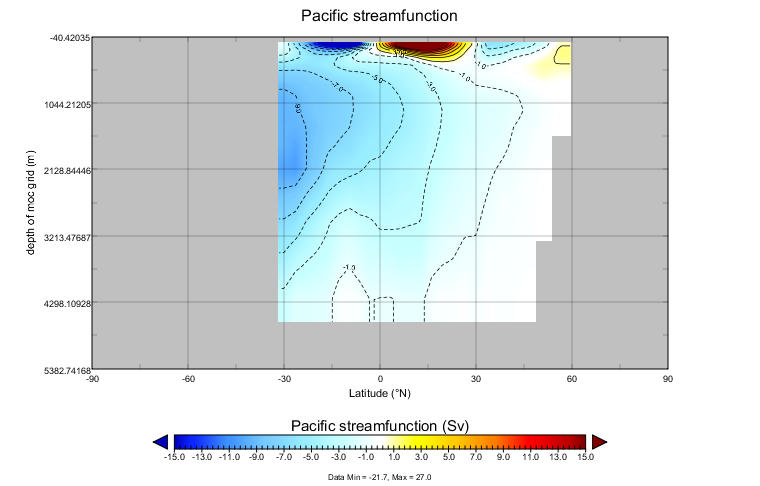
\includegraphics[width=0.6\textwidth]{ch3-amoc2.png}\centering
\vspace{-0mm}
\caption{Pacific meridional overturning circulation (PMOC).}
\label{fig:ch3-amoc2}
\end{figure}

%------------------------------------------------
\newpage
%------------------------------------------------

\section{Tracing ocean circulation}

The ocean biogeochemistry module (\textbf{BIOGEM}) in \textbf{muffin} provides a framework for applying time- and spatially-variable ‘forcings’ of the Earth system\footnote{Refer to the '\textit{force the system}' \textsf{HOW-TO} in the muffin manual for further details on \textit{forcings}.} – fluxes or 'restored-to' boundary conditions that can be prescribed for any gas, dissolved substance (including temperature and salinity), or particulate matter. Examples include freshwater input (== a negative salinity flux forcing) of the North Atlantic to alter ocean circulation, fossil fuel \(CO_{2}\) emissions to the atmosphere (== a \(CO_{2}\) gas flux forcing), or aeolian iron supply to the surface ocean (a 2-D dust flux forcing).

\vspace{1mm}
For example: view the \textit{user-config} file: \textsf{\footnotesize LAB\_2.colorinjection} – you will see the following lines (under the heading: ‘\texttt{\# --- FORCINGS ---}’)

\vspace{-2mm}\small
\begin{verbatim}
bg_par_forcing_name="pyyyyz_Fred"
bg_par_force_point_i=22
bg_par_force_point_j=33
bg_par_force_point_k=8
bg_par_ocn_force_scale_val_48=0.0
\end{verbatim}
\normalsize\vspace{-2mm}

The first line points \textbf{muffin} to a directory located in \textsf{\footnotesize cgenie.muffin/genie-forcings} that contains a set of files that define what geochemical property is going to be altered plus information about how the magnitude of the forcing changes with time.

There are then three lines (\texttt{bg\_par\_force\_point\_i=20}, ...) that specify the location in the ocean of the geochemical forcing that is going to be applied. The point sources are specified in (i,j,k) coordinates, which in this case is (22,33,08). For the ocean model resolution we are using, the grid is 36x36x16, and in which: longitude (i) is counted from left-to-right (1 to 36); latitude (j) is counted from bottom-to-top (1 to 36); level depth (k) is counted from downwards top-to-bottom (16 down to 1). Thus, (22,33,08) is a release of tracer in the North Atlantic, a little south of Greenland, and intermediate depth (level = 8 out of 16). Refer to the Figures for how the horizontal (Figure \ref{fig:ch3-ijgrid}) and vertical (Figure \ref{fig:ch3-kgrid}) grid is specified.

Finally, there is a scaling parameter (\texttt{bg\_par\_ocn\_force\_scale\_val\_48}) which modifies the magnitude of the flux to be applied (in units of \(mol yr^{-1}\) per model grid point).

%------------------------------------------------
\newpage 
%------------------------------------------------

%
\begin{figure}
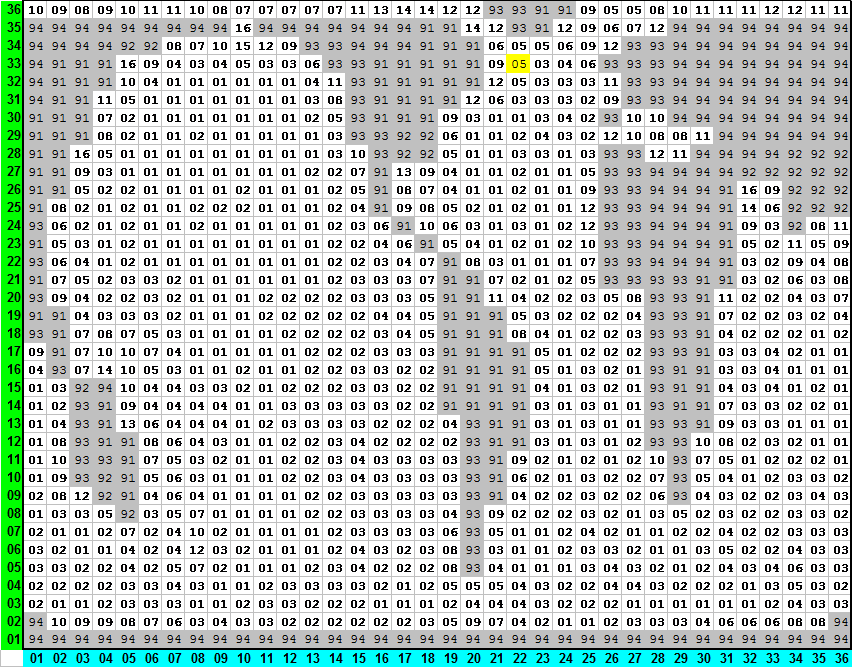
\includegraphics[width=0.8\textwidth]{ch3-ijgrid.png}\centering
\vspace{-0mm}
\caption{
\textbf{The  muffin grid for a modern \(36\times36\) ‘worjh2’ configuration.} Light blue numbers are the ‘i’ co-ordinates. Green numbers are the ‘j’ co-ordinates.
The depth of the ocean at any location is indicated by its ‘k’ value – a number between 1 and 16, with 16 being the surface layer of the ocean, and 1 the maximum possible depth anywhere.
Numbers > 90 (91, 92, 93, 94) and shaded grey are land (and specify the direction of run-off).
Location (22,33,08) is highlighted in yellow.
The longitude of the western edge of this particular modern ocean grid is at 260W, and the increments are 10 degrees.
}
\label{fig:ch3-ijgrid}
\end{figure}

\begin{figure}
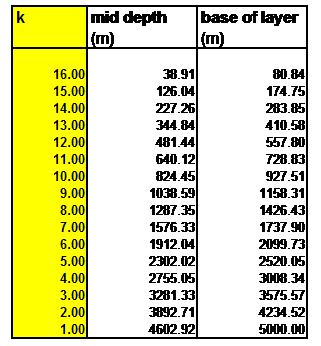
\includegraphics[width=0.4\textwidth]{ch3-kgrid.png}\centering
\vspace{-0mm}
\caption{\textbf{The muffin ocean vertical level definitions for a modern 16-level ocean grid.}}
\label{fig:ch3-kgrid}
\end{figure}

\noindent You are going to run a brief experiment in which you will be injecting a conservative ‘dye’ tracer into the ocean. The \textbf{BIOGEM} module has two tracers defined for this purpose – ‘blue’ and ‘red’. Open the \textit{user-config} file: \textsf{\footnotesize LAB\_2.colorinjection} and edit the parameter controlling the flux of red dye to read:

\vspace{-2mm}\small
\begin{verbatim}
bg_par_ocn_force_scale_val_48=1.0E12
\end{verbatim}
\normalsize\vspace{-2mm}

\noindent which specifies a flux of \(1.0\times10^{12}\) ( \(mol yr^{-1}\)) rather than zero as given as the default in the example \textit{user-config} file\footnote{i.e. don't leave the value as zero ... otherwise you'll have no flux forcing applied and will not see anything happen ...}.

\vspace{1mm}
The \textit{base-config} you will be using is different from previously: \textsf{\footnotesize cgenie.eb\_go\_gs\_ac\_bg.worjh2.rb} – this specifies a 16 vertical levels ocean and also includes seasonality of solar insolation.\footnote{Note that because the \textit{base-config} is different from that used in the previous chapter, you need to force a re-compile of the model code before any experiments can be submitted as cluster jobs. The easiest way to do this is to run an experiment interactively at the command line.}

%------------------------------------------------
\vspace{1mm}
\noindent\rule{4cm}{0.5pt}
\vspace{2mm}
%------------------------------------------------

%------------------------------------------------
\newpage 
%------------------------------------------------

\noindent Run the model for … whatever, 20 years will do. Use the \textit{re-start} experiment that you have just downloaded to start from:

\vspace{-2mm}\small
\begin{verbatim}
$ ./runmuffin.sh cgenie.eb_go_gs_ac_bg.worjh2.rb LABS LAB_2.colorinjection 20 LAB_2.SPIN
\end{verbatim}
\normalsize\vspace{-2mm}

View the results – for instance how the red tracer distribution evolves with time – in the \textit{time-slice} files (full ocean/atmosphere) properties saved in the \textbf{netCDF} format (\texttt{.nc}) files). You can follow the progress of the dye (and hence diagnose the properties of ocean circulation in the model) by plotting vertical and/or horizontal slices that go through (or near) the cell location in which you inject the dye tracer in the 3D \textbf{netCDF} file. Note that \textbf{Panoply} appears to ‘count’ the ocean layers in the opposite direction to the way in which the ocean model is actually counting them – the correct definition is with ‘1’ being very deepest level possible (and as displayed in the figure) and '16' is the surface.

You can also view the tracer distributions in terms of a water-column integrated tracer inventory (\textbf{netCDF} variable name: \textsf{\footnotesize ocn\_int\_colr}; long name: \textsf{\footnotesize colr water-column integrated tracer inventory}) in the 2D \textbf{netCDF} output. (See: \textit{Sabine et al.} [2004] for the use of water column integrals in the context of the distribution of anthropogenic \(CO_{2}\) uptake and storage.) Changes in tracer inventory with time can be tracked in the time-series file:

\vspace{-2mm}\small
\begin{verbatim}
biogem_series_ocn_colr.res.
\end{verbatim}
\normalsize\vspace{-2mm}

Spend a little while altering the flux (\texttt{\small bg\_par\_ocn\_force\_scale\_val\_48}) and/or location
\\(\texttt{\small bg\_par\_force\_point\_i}, \texttt{\small bg\_par\_force\_point\_j, bg\_par\_force\_point\_k}) of tracer input. Overall -- note how you can use numerical ‘tracers’ to help diagnose (and better understand) the circulation of the ocean.

%------------------------------------------------
\vspace{1mm}
\noindent\rule{4cm}{0.5pt}
\vspace{2mm}
%------------------------------------------------

%------------------------------------------------
\newpage 
%------------------------------------------------
%
\noindent When you add the numerical dye, particularly early on in the experiment, you may see a 'front' of \uline{negative} tracer concentrations leading the (positive) tracer as it spreads. DON'T PANIC!

The model is ... a model (of the numerical flavor) and not an exact analytical solution. So errors in how it solves ocean transport are to be expected.

Moreover, by default the ocean circulation model employs an isopycnal/diapycnal mixing scheme. This can lead to unwanted negative tracer values when sharp horizontal (or vertical) transitions in concentration occur. (In this example, e.g. by injection dye at a point location into a surrounding ocean of initially zero concentration.)

You can change to a simpler horizontal/vertical (.false.) mixing scheme by adding to the \textit{user-config} file:

\vspace{-2mm}\small
\begin{verbatim}
# turn OFF (=.false.) isopycnal/diapycnal mixing
go_diso=.false.
\end{verbatim}
\normalsize\vspace{-2mm}

If you try this, you should (hopefully) find much less (or no) negative tracer concentrations occur. However, also note that by changing the physics of ocean mixing, you also slightly alter the large-scale circulation of the ocean (and e.g. the AMOC might change slightly in strength).\footnote{You might contrast the overturning stream-functions for experiments run both with and without horizontal/vertical mixing.} 

%------------------------------------------------
\vspace{1mm}
\noindent\rule{4cm}{0.5pt}
\vspace{2mm}
%------------------------------------------------

\noindent Lastly, an interesting (honest!) and illustrative exercise is to use the dye tracer to pick out the path taken by Mediterranean Intermediate Water. Despite the low resolution of the \textbf{muffin} ocean circulation model component and the highly restricted representation of the Mediterranean, the model does project a salty Mediterranean as a consequence of  P-E across this basin (and its catchments) being negative and this higher density water makes its way out in the subsurface into the Atlantic.

To do this -- simply specify a dye injection somewhere in the Mediterranean (be careful with the restricted depth of the Mediterranean – if you inject too deeply (into the crust!) then you will not see anything (refer to the figure for the depth level (k) number of the maximum depth of the water column in each location), and it is better to inject it relatively close to the opening of the gateway (try some different locations and see which ones produce a reasonably instructive tracing of Mediterranean outflow). Run for e.g., 20 or 50 years (from the provided spin-up). Then:

\vspace{1mm}
\begin{enumerate}[noitemsep]
\vspace{1mm}
\item View the dye-tagged plume of Mediterranean Intermediate Water by plotting a lat-lon slice (from the 3D \textbf{netCDF} file). This will give you the depth of the plume. How does this compare with salinity observations (salinity observations and appropriate global data-sets can be found on the web with a little patience)? You can also view the water-column integrated distribution (2D \textbf{netCDF}).
\vspace{1mm}
\item Try viewing the plume via a lat-depth slice. Refer to the figure to determine the ‘i’ value up the Atlantic that will just graze the edge of what passes for Spain at this low model resolution. Which direction does it head after exiting the Mediterranean? Is this ‘realistic’?
\end{enumerate}
\vspace{1mm}

%------------------------------------------------
\newpage
%------------------------------------------------

\section{Tracing ocean ... ventilation}

Yet another way to think about global ocean circulation is through considering the connection (rate of mass exchange) between surface and deep ocean -- 'ventilation'.

\textbf{muffin} has the capability to employ/simulate a ventilation age tracer\footnote{Under the '\textit{screw with and/or diagnose the climate system}' HOW-DO -- see '\textit{Add a water mass age tracer}' (and the 'easy'/automatic method described towards the end of that section).} -- a numerical tracer carried in the ocean circulation model that tracks the time since a parcel of water last 'saw' the surface. The older the 'age' of the parcel of water, the longer the time since it last saw the surface.

We can use the same 'red' numerical tracer to keep track of age, but rather than apply a flux forcing to the surface, we let the model automatically restore the tracer value at the surface to zero and everywhere else (in the ocean interior) increase the age each time-step (by the duration of the time-step) such that a parcel of water away from the surface ages by 1 year, each year.

%------------------------------------------------
\vspace{1mm}
\noindent\rule{4cm}{0.5pt}
\vspace{2mm}
%------------------------------------------------

\noindent Provided is a  \textit{user-config} file for including an age tracer in the model: \textsf{\footnotesize LAB\_2.age}. You will also need a new \textit{re-start} experiment, called: \texttt{muffin.C.p\_worjh2.r.SPIN} and which can be downloaded and unpacked as per before (both from \textsf{\footnotesize cgenie\_output)}:

\vspace{-1mm}\small
\begin{verbatim}
$ wget --no-check-certificate 
     http://www.seao2.info/cgenie_output/muffin.C.p_worjh2.r.SPIN.tar.gz
\end{verbatim}
\normalsize\vspace{-1mm}
(all one line) and then:
\vspace{-1mm}\small
\begin{verbatim}
$ tar xfzv muffin.C.p_worjh2.r.SPIN.tar.gz
\end{verbatim}
\normalsize\vspace{-1mm}

To run (e.g. for 10 years), following on from its \textit{re-start} experiment, would be:

\vspace{-1mm}\small
\begin{verbatim}
$ ./runmuffin.sh cgenie.eb_go_gs_ac_bg.worjh2.rb LABS LAB_2.age 10
     muffin.C.p_worjh2.r.SPIN
\end{verbatim}
\normalsize\vspace{-1mm}

In the 3D netCDF output file -- \textsf{\footnotesize misc\_col\_Dage} is the output variable that is the calculated ventilation age.

Explore the distribution of water mass age and think about the physical ocean circulations reasons for this. Are all the modelled distributions reasonable? Are there indicators of facets of the simulated circulation that are not particularly realistic? Try plotting both lon-lat and lat-depth slices through the ocean. How does the distribution of water mass age relate to the overturning stream-function for Atlantic or Pacific basins (more on this in the next Section)?

%------------------------------------------------
\newpage
%------------------------------------------------

\section{Poking the climate beast}

Instead of adding a dye tracer, you could add fresh water to the ocean surface to assess the sensitivity of the Atlantic Meridional Overturning Circulation (AMOC) to collapse, in a classic ‘hosing’ experiment.

The \textit{user-config} file for this is called: \texttt{LAB\_2.hosing}. The default (i,j) location of the flux input is the same (as the dye tracer), but now the injection at the surface (level: k=16). Note that the forcing of the salinity tracer is negative (freshwater = negative salinity compared to sea-water)!

To orientate you in freshwater forcing space: \texttt{bg\_par\_ocn\_force\_scale\_val\_2=-2.0E17} should be sufficient to make ‘stuff happen’ and quickly. BUT, this is a pretty extreme flux (see overleaf for a rough conversion between salinity forcing units (mol yr$^{-1}$) and fresh water flux (in m$^{3}$ s$^{-1}$ or Sv). Much more than this and the model may crash or at the very least, you’ll be left with a large freshwater pond in the North Atlantic … (see later for some exciting discussion on units!)

\vspace{1mm}
To run the model for e.g., 20 years using the same restart:

\vspace{-2mm}\small
\begin{verbatim}
$ ./runmuffin.sh cgenie.eb_go_gs_ac_bg.worjh2.rb LABS LAB_2.hosing 20 LAB_2.SPIN
\end{verbatim}
\normalsize\vspace{-2mm}

\noindent 20 years should be long enough to see a collapse start to occur, but you might want to run the model for longer (and it can be submitted as a job, of course). Running for longer will also allow you to have a smaller, less extreme (and maybe more realistic) freshwater input flux.

Make sure that you run a \uline{control} experiment -- an experiment of the same duration of your hosing experiments, but with a zero freshwater flux. The impact of freshwater input, is the difference, at the same model year, between the perturbation experiment and the control. (You only ever need need to run one control, regardless of how many different freshwater flux perturbation experiments  you run.) 

Note that as the model is running rather s l o w e r than in the snowball configuration, you might want to think carefully of making use of cluster queuing possibilities (i.e., running multiple experiments at once in the background).

%------------------------------------------------
\vspace{1mm}
\noindent\rule{4cm}{0.5pt}
\vspace{2mm}
%------------------------------------------------

\noindent The most obvious property of the Earth system to follow is the Atlantic overturning strength (\textsf{\footnotesize biogem\_series\_misc\_opsi.res}). The AMOC stream-function (in \textsf{\footnotesize fields\_biogem\_2d.nc} 2-D time-slice \textbf{netCDF} results file, field: \textsf{\footnotesize phys\_opsia}) is also illustrative. You can also try and identify the salinity anomaly (see below) due to freshwater input in the 3D salinity tracer field.

There are also important (but not necessarily painfully exciting) impacts on surface air temperatures and maybe sea-ice extent (in \texttt{fields\_biogem\_2d.nc)} (but see below for a better way to visualize these changes). Note the importance (sort of) of the AMOC in transporting heat to the N Atlantic region (the film the Day After Tomorrow was not entirely inaccurate in this particular respect). Be aware of the possibility of climate impacts far from the location of fresh water forcing. Look out for any significant-looking impacts on sea-ice extent, etc.

You might also plot current velocity fields and visualize how these change in response to the fresh water forcing. 

%------------------------------------------------
\vspace{1mm}
\noindent\rule{4cm}{0.5pt}
\vspace{2mm}
%------------------------------------------------

%------------------------------------------------
\newpage
%------------------------------------------------

\noindent To more easily assess some of these impacts (and for other sorts of analysis) it is possible to create an \uline{anomaly (difference) map} in \textbf{Panoply}:

\vspace{1mm}
\begin{enumerate}[noitemsep]
\vspace{1mm}
\item  First open a dataset, e.g., \textsf{\footnotesize atm\_temp} (surface air temperature) in the 2D \textbf{netCDF} file. You can either double-click the variable name, or, with the variable name highlighted, click the ‘Create Plot’ icon.
\vspace{1mm}
\item Now, with the \textsf{\footnotesize atm\_temp} still selected (and the first plot window still open), click on the ‘Combine Plot’ icon. A dialogue box will appear and ask you to select a plot to combine the new one with. Make sure the name of your first plot window is selected/highlighted. Click ‘Combine’. OR, simply drag a second dataset into the plot window of the first dataset.
\vspace{1mm}
\item You now have a plot window that by default it is showing you the difference between two identical (in time) slices. The two different slices are labeled Array 1 (LH side) and Array 2 (RH side).
\end{enumerate}
\vspace{1mm}

Keep one array (Array 1) fixed to the initial (year 1 (centered on 0.5)) and vary the year in the second array (Array 2). Note that you can select in Panoply whether Array 1 – Array 2 is plotted, or Array 2 – Array 1, or various proportional or relative differences.

Note that you can switch off the auto-scaling feature (Always fit to data) and center the scale so that no change is white, with positive deviations = red and negative = blue by clicking on Center on 0 (an often used convention in climate field plotting).

%------------------------------------------------
\vspace{1mm}
\noindent\rule{4cm}{0.5pt}
\vspace{2mm}
%------------------------------------------------

\noindent Finally, a brief note on units ... the freshwater forcing is implemented as negative salinity, just to really screw with your mind. The generic internal \textbf{muffin} model units for the forcing end up as \(PSU kg^{-1} yr^{-1}\). Which sort of does not make much sense ...

Start, by thinking of a value of \texttt{bg\_par\_ocn\_force\_scale\_val\_2} of \(-34.9\) as equivalent to taking all the salt out of \(1 kg\) of freshwater (since the mean global salinity is \(34.9 PSU\)). Or equivalently, since the ocean volume is fixed, an applied forcing value of \(-34.9\) is equivalent to adding \(1 kg\) of freshwater to a (surface) box. So, a value of \texttt{bg\_par\_ocn\_force\_scale\_val\_2} of \(-3.49\times10^{4}\) (\(-3.49E04)\) would be a flux of \(1 m^{3} yr^{-1}\) (\(1000 kg m^{-3}\)) of freshwater.

So, in the example earlier (\texttt{bg\_par\_ocn\_force\_scale\_val\_2=-1.0E18}), the freshwater flux is \(1.0\times10^{18}/3.49\times10^{4} = 2.8653\times10^{13} m^{3} yr^{-1}\).

The literature invariably gives freshwater fluxes in units of \(Sv\) (\(10^{6} m^{3} s^{-1}\)). So in the example, the freshwater flux is: \(9.0797\times10^{5} m^{3} s^{-1}\) (\(365.25\times24\times3600 = 31557600 s yr^{-1}\)). Or \(0.9 Sv\).

Or or ... \(1.0 Sv\) is equivalent to a model (\texttt{bg\_par\_ocn\_force\_scale\_val\_2}) total forcing flux of \(-1.0E18/0.90797 = -1.1E18\)

Read the literature … but generally, fluxes of ca. \(0.05 Sv\) and larger (and to quite specific places) are applied in models to induce an AMOC collapse.

%------------------------------------------------
\newpage
%------------------------------------------------

\section{Further ideas}

%------------------------------------------------

\subsection{Hosing investigations}

What is the largest freshwater flux that can be sustained without ‘collapsing’ the AMOC? Is there a ‘threshold’ (‘tipping point’) of freshwater input, beyond which the AMOC rapidly decreases in strength? For this -- you would run (submit to the cluster) a series of experiments, each with different (increasing) values for the fresh water flux. Remember to include an experiment with zero freshwater flux to act as a 'control'.

Is the precise location of the freshwater input important (i.e., try tipping it in somewhere else)? For this -- you could piece-meal run an experiment, analyse the results, then choose a new location to input the freshwater, or, come up with a systematic search pattern of freshwater input patterns.  

Outside of the North Atlantic, are any other  regions (of deep water formation) sensitive to freshwater perturbation and what are the consequences (could it happen in the future)?

%------------------------------------------------

\subsection{‘Anti-hosing’ investigations}

There are questions concerning past changes in the AMOC as to whether it is ‘pushed’ or ‘pulled’. i.e., if the AMOC shoals in depth and/or weakens, is it because its production has weakened, or as Antarctic Bottom water (AABW) strengthened and ‘pushed’ it out of the way (to shallower depths)?

What you might try then is to inject salt in the Southern Ocean as opposed to fresh water in the North Atlantic. All you need do is pick an appropriate grid point (this is worth thinking about carefully and maybe testing different locations) and rather than giving the parameter \texttt{bg\_par\_ocn\_force\_scale\_val\_2} a negative value, you give it a positive one. (Start by trying similar magnitudes of value as before and see what happens.)

\textbf{Is the AMOC (for the same magnitude of forcing) more sensitive to being ‘pushed’ or ‘pulled’?} (Obviously the answer will  depend on where the perturbations are being applied.)

%------------------------------------------------

\subsection{Response to transient warming}

A current concern regarding anthropogenic climate change is the ocean circulation (and marine ecological and biogeochemical) response to a strong warming of the surface, as rapid surface warming is assumed (and demonstrated in models) to result in surface stratification of the ocean, likely restricting the nutrient supply to phytoplankton and reducing ventilation of the ocean interior with dissolved oxygen.

You can explore the transient response of ocean circulation to warming by simply adjusting the radiative forcing parameter as per used in the snowball Earth experiments: \texttt{ea\_radfor\_scl\_co2}. By default in the modern continental configuration, this has a value of 1.0, corresponding to 278 ppm atmospheric \(CO_{2}\). A value of 2.0 would reflect warming equivalent to 556 ppm \(CO_{2}\). And 3.0 more like an end-of-the-century warming. Note that you are applying the warming instantaneously by manipulating the climate system in this way and hence the changes will be more extreme than those occurring over the time-scale of this century. Also note that a cooling could be applied instead. A \textit{user-config} –- \textsf{\footnotesize LAB\_2.EXAMPLE} – is provided as a template for these experiments.

Potentially interesting properties of the Earth system to look at include sea-ice extent and AMOC strength (in the ASCII time-series files), and the overturning stream-function and sea-ice extent in the 2-D \textbf{netCDF} output. It is also possible to fresh water force the model with an age tracer and hence make projections of how patterns of ventilation age change with transient warming.

Overall, try and answer the question: \textbf{How much radiative forcing is required to collapse the AMOC? What atmospheric \(CO_{2}\) value does this approximately correspond to?}

%----------------------------------------------------------------------------------------
%----------------------------------------------------------------------------------------